% CVPR 2022 Paper Template
% based on the CVPR template provided by Ming-Ming Cheng (https://github.com/MCG-NKU/CVPR_Template)
% modified and extended by Stefan Roth (stefan.roth@NOSPAMtu-darmstadt.de)

\documentclass[10pt,twocolumn,letterpaper]{article}

%%%%%%%%% PAPER TYPE  - PLEASE UPDATE FOR FINAL VERSION
%\usepackage[review]{cvpr}      % To produce the REVIEW version
\usepackage{cvpr}              % To produce the CAMERA-READY version
%\usepackage[pagenumbers]{cvpr} % To force page numbers, e.g. for an arXiv version

% Include other packages here, before hyperref.
\usepackage{graphicx}
\usepackage{amsmath}
\usepackage{amssymb}
\usepackage{booktabs}


% It is strongly recommended to use hyperref, especially for the review version.
% hyperref with option pagebackref eases the reviewers' job.
% Please disable hyperref *only* if you encounter grave issues, e.g. with the
% file validation for the camera-ready version.
%
% If you comment hyperref and then uncomment it, you should delete
% ReviewTempalte.aux before re-running LaTeX.
% (Or just hit 'q' on the first LaTeX run, let it finish, and you
%  should be clear).
\usepackage[pagebackref,breaklinks,colorlinks]{hyperref}


% Support for easy cross-referencing
\usepackage[capitalize]{cleveref}
\crefname{section}{Sec.}{Secs.}
\Crefname{section}{Section}{Sections}
\Crefname{table}{Table}{Tables}
\crefname{table}{Tab.}{Tabs.}


%%%%%%%%% PAPER ID  - PLEASE UPDATE
\def\cvprPaperID{*****} % *** Enter the CVPR Paper ID here
\def\confName{CVPR}
\def\confYear{2022}


\begin{document}

%%%%%%%%% TITLE - PLEASE UPDATE
\title{Team 4 - Preliminary Project Report}

\author{Tadipatri Uday Kiran Reddy\\
{\tt\small ee19btech11038@iith.ac.in}
% For a paper whose authors are all at the same institution,
% omit the following lines up until the closing ``}''.
% Additional authors and addresses can be added with ``\and'',
% just like the second author.
% To save space, use either the email address or home page, not both
\and
Sahukari Chaitanya Varun\\
{\tt\small ee19btech11040@iith.ac.in}
\and
L. Pranay Kumar Reddy\\
{\tt\small ai19btech11019@iith.ac.in}
}
\maketitle

%%%%%%%%% ABSTRACT
\begin{abstract}
With the evolution of high-resolution digital cameras, snapshots have become the most common way to record and share visual data and experiences taken through mobile phones and tablets. But as humans, it is challenging to keep a stiff hold while capturing an image, especially when the image is to be captured on the move; it introduces blur. Though there lot of external tools for frame stabilization, such as gimbal, mounting it on can be challenging at times. Hence, we propose this paper to solve this problem by processing the image with the aid of gyroscope sensed data  attached with the camera device, helping to deblur the image. We aim to implement this deblurring with the help of deep convolution nets and extrapolate it with GAN's to give better quality and faster output than  traditional CNN's. We can extend this work to stabilise the video feed with lower frame rates with faster computation capabilities.
\end{abstract}

%%%%%%%%% BODY TEXT
\section{Introduction}
\label{sec:intro}
% Introduce the problem you are working on. This section should give a general introduction motivation for the problem. You can also describe the applications of your problem here. 

% Please number all of your sections and displayed equations as in these examples:
% \begin{equation}
%   E = m\cdot c^2
%   \label{eq:important}
% \end{equation}
% and
% \begin{equation}
%   v = a\cdot t.
%   \label{eq:also-important}
% \end{equation}
Our desired scenes are always in motion; capturing this in the camera would introduce a fuzzy noise known as motion blur. This effect is also very severe in Autonomous vehicles which utilise sophisticated visual SLAM algorithms on live feed coming from cameras or LIDAR sensors that are in motion. Here the motion blur would suppress the crucial features needed to be obtained from the video feed. Even with state-of-the-art technology of camera manufacturing, the motion blur effect is not being improved while the camera resolution is getting better and better.\\

Mechanically stabilising the sensor like camera or LIDAR is very hard, so we have to use rigorous algorithms to process the image and many recent works like {} came up with both linear and non-linear models to deblur the image but the processed images are having still some blur and implementation of such sophisticated algorithm in edge devices like mobile phones, DSLR cameras, etc is computationally infeasible. These works leave the fact behind that these motion blurs are caused due to relative motion between scene and camera. As all the modern mobile phones and camera are equipped with Interial Measurement Units(\textit{IMU}), these actually measure velocity, acceleration, we can exploit this sensor data to deblur the images than only using raw image only as data. These \textbf{works} actually can up with system to exploit gyroscope sensor data, here they use Convonutaional Neural Network(CNN) with encoder and decoder framework, but these demand high computational power.\\

In this work we propose a framework which deblurres images with blurred image and gyroscope sensor data, with help of deep-CNN and extrapolate it with Generative Adversarial Network(\textit{GAN}) to enchance the quality and faster output of deblurred image.\\
The below are the main contribution of this paper.
\begin{enumerate}
	\item We propose a framework known as Motion blur Correction with Gyroscope using Generative Adverserial Networks(\textit{MCG-GAN})
	\item We use MCG-GAN for deblurring images and show the improvement with existing state-of-art-works.
\end{enumerate}
The rest of the paper is organised as follows - We discuss the detailed problem statement in Section 2. We provide literature review in Section 3 which describes the related works and mentions important results which are going to be used in proposed framework. In section 4, we show results of recent works on deblurring. Finally, in section 5, We cite the references from we have used or described the paper.
%------------------------------------------------------------------------
\section{Problem Statement}
\label{sec:problem}
The problem statement concisely is image deblurring aided by gyroscopic sensing implemented through GAN's, building upon the deep neural net solution. Though the blur introduced can be from relative motion between the camera and picturing object itself, we focus only on deblurring image due to the relative movement of the camera device.\\
The paper DeBlurGAN has already produced a benchmark result in finding the blur and rectifying it, but assumes the blur to be space invariant, i.e, performs blind deblurrring over the whole image. We can at first estimate a spatially variant motion field and blur kernels from a single image using deep networks, thereafter perform non-blind deconvolution. But often, this process requires input of multiple images which might not always be available. We here focus on single image deblurring approach. \\

From the gyroscopic measurements, the rotation can be estimated as
\begin{equation}
    \frac{d \textbf{q(t)}}{dt} = \frac{1}{2}\textbf{q(t)} \bigodot \omega(t), \textbf{q(t1)=1}
\end{equation}
where $\omega$(t) is the 3-dimensional gyroscope measurement and $\bigodot$ denotes the quaternion product. The initial condition is given at the starting time of exposure t1 and the solution is computed at the end time of exposure t2.
The motion blur caused by translation will depend on the scene depth, which is difficult to estimate from a single image and hence take these limitations into account when generating training data. Consider $\textbf{R(t)}$ and $\textbf{t}$(t) as rotation and translation of camera. Assuming the scene depth to be a constant $\textbf{d}$ , the motion of camera can be modeled as planar homograph as :
\begin{equation}
    \textbf{H(t)} = \textbf{K[R}(t) - \frac{\textbf{t}(t)\textbf{n}^{T}}{d}\textbf{]K}^{-1}
\end{equation}
where K is the intrinsic camera matrix obtained via calibration. By taking the translation to be zero, this simplifies to 
\begin{equation}
    \textbf{H(t)} = \textbf{KR}(t)\textbf{K}^{-1}
\end{equation}
By this we can compute the blur vector for every pixel, which gives us the blur map of the image \textbf{h}.

Now, as we have a blurred image $I_{\textbf{b}}$, our goal is to predict a sharp image I using GANs, such that 
\begin{equation}
I_{\textbf{b}} = \textbf{h}*I + \textbf{n}
\end{equation}
where h is the kernel which models the motion blur also called as blur kernel, n is the noise and * denotes convolution.

\section{Literature Review}
\label{sec:literature}
\subsection{Motion blur}
This is a phenomenon observed in images taken when there is relative motion between camera and the scene, these are the artifacts observes in most common camera which are mostly rolling shutter cameras. Many of the recent works model the motion blur as Linear Space invariant system as follows.
\begin{equation}
I_{\textbf{b}} = \textbf{h}*I + \textbf{n}
\end{equation}
Where $I_{\textbf{b}}$ is Blurred image, \textbf{h} is kernal which models the motion blur more ofently so know as Point Space Function(\textit{PSF}), I is actual unblurred image and finally \textbf{n} is noise added while capturing the snap.\\

In this paper, we use gyroscope data and take into consideration that blur kernel is space variant.
\begin{equation}
I_{\textbf{b}} = f\left(I, \textbf{g}(\textbf{t}), \textbf{n}\right)
\end{equation}
Where f(\textbf{.}) is non-linear space invariant function, this is learnt from dataset using GANs which is further more discussed in Section 3.3.
\subsection{DeepGyro}
The deblurring is based on fully-convolutional neural network which aims to produce a shar image given blurred image and gyro-based blur field. The netwrok architecture is similar to encoder-decoder network, where the input network consists of blurred RGB image and a gyro-based blur field which pass through series of convolutional and downsampling layers until the lowest resolution is reached. After the bottleneck, this low resolution image is expanded back into a full resolution image with help of upsampling layers. Skip connections are used to allow information sharing between encoder and decoder.\\
For training of data, the blurred and sharp images with gyro-based blur fields are produced by taking the visual-inertial dataset which consists of various types camera motion resulting in different blur fields. The blur fields are themselves further distorted to exact and noisy blur fields for training a robust model. The paper states of utilizing nearly 100k images and was evaluated on both synthetically and naturally blurred images.
\\

In regard to the current paper we are working on, this refered paper serves as model for extracting the gyro data and also  help in generating the datasets required for training and testing the model. This model is embedded in initial stages of our model which is then build further by GANs.

\subsection{Generative adversarial networks (GANs)}
Generative adversarial networks (GANs), introduced by Ian Goodfellow provides a way to learn deep representations without extensively annotated training data. They achieve this through deriving back-propagation signals through a competitive process also called min-max game involving a pair of networks known as the discriminator and the generator. 
\\

The generator receives noise as an input and generates a sample. A discriminator receives a real and generated sample and is trying to distinguish between them. The goal of the generator is to fool the discriminator by generating perceptually convincing samples that can not be distinguished from the real one. The game between the generator G and discriminator D is the minimax objective:
\begin{equation}
min_{G} max_{D} E_{x \sim P_{\textbf{r}}}[log(D(x))] + E_{z \sim P_{\textbf{g}}}[1 - log(D(G(z)))]
\end{equation}\textbf{}

where $P_{\textbf{r}}$ is the data distribution and $P_{\textbf{g}}$ is the model distribution, defined by z $\sim P_{z}$, the input z is a sample from a simple noise distribution

\section{Preliminary Results}
\label{sec:prelim_results}
\subsection{DeepGyro}
\vspace{-0.5cm}
\begin{figure}[h]
    \centering
    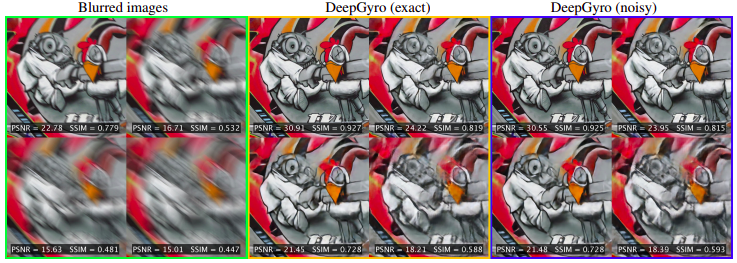
\includegraphics[width=2.2\columnwidth,height=6cm]{images/deepgyro.png}
    \caption{ DeepGyro performance for increasing levels of blur, Blurred images (green)}
    \label{fig: result_deepgyro}
\end{figure}

%-------------------------------------------------------------------------
\section{References}
\begin{enumerate}
    \item \href{https://arxiv.org/abs/1810.00986}{Gyroscope-Aided Motion Deblurring with Deep Networks}, Janne Mustaniemi, Juho Kannala, Simo Särkkä, Jiri Matas, Janne Heikkilä
    \item \href{https://arxiv.org/abs/1406.2661}{Generative Adversarial Networks},
Ian J. Goodfellow, Jean Pouget-Abadie, Mehdi Mirza, Bing Xu, David Warde-Farley, Sherjil Ozair, Aaron Courville, Yoshua Bengio
    \item \href{https://arxiv.org/abs/1711.07064}{DeblurGAN: Blind Motion Deblurring Using Conditional Adversarial Networks},
Orest Kupyn, Volodymyr Budzan, Mykola Mykhailych, Dmytro Mishkin, Jiri Matas
\end{enumerate}


%%%%%%%%% REFERENCES
{\small
\bibliographystyle{ieee_fullname}
\bibliography{egbib}
}

\end{document}
